\documentclass[11pt]{article}

\usepackage[margin=1in]{geometry}
\usepackage{amsmath,amssymb}
\usepackage{graphicx}
\usepackage{booktabs}
\usepackage{array}
\usepackage{nicematrix}
\usepackage[labelfont=bf]{caption}
\usepackage{natbib}
\usepackage{hyperref}

\title{Geodesic Beam Search: A Modular Method for Discovering\\
Novel Chaotic Attractors in Polynomial Vector Field Space}
\author{%
\begingroup
\setlength{\tabcolsep}{0pt}
\begin{tabular}{>{\centering\arraybackslash}p{0.48\textwidth}>{\centering\arraybackslash}p{0.48\textwidth}}
Isaac Dash & Dr. William Hahn \\[4pt]
\textit{Undergraduate Researcher} & \textit{Associate Professor} \\
\textit{Department of Mathematics} & \textit{Department of Mathematics and Statistics} \\
\textit{New York University} & \textit{Florida Atlantic University}
\end{tabular}%
\endgroup
}
\date{}

\begin{document}
\maketitle

\begin{abstract}
We present \emph{Geodesic Beam Search}, a method for systematically discovering
novel three-dimensional chaotic attractors within the space of quadratic
polynomial vector fields. Starting from a curated set of known chaotic systems
represented as unit vectors in an 81-dimensional coefficient space, the method
iteratively expands a frontier of ``seed'' systems by stepping out along
equiangular tangent directions via exact geodesics at several fixed arc-lengths,
discards candidates that fall too close to already-cataloged territory, and
retains only the top-ranked most chaotic new discoveries each round as the next
round's seeds. This beam-search-style capping rule keeps per-round
computational cost roughly constant rather than compounding. Crucially, the
search framework itself is decoupled from the two decision procedures it
depends on: a \emph{chaos oracle}, which classifies whether a candidate system
is genuinely chaotic and supplies a fitness score for beam selection, and a
\emph{novelty oracle}, which decides whether a chaotic hit is
distinct from all chaotic systems cataloged so far. Either oracle can be
replaced without modifying the search mechanics. Applying the method for 15
rounds, seeded from 36 known attractors and using a multi-draw
Lyapunov-exponent/correlation-dimension chaos oracle together with a
Zernike-moment/ICP shape-alignment novelty oracle, we evaluate approximately
394{,}000 candidate coefficient vectors, identify approximately 27{,}500
chaotic hits, and confirm 12{,}200 as geometrically distinct from every other
known or discovered system. We characterize the resulting yield dynamics,
discuss limitations, and outline applications to forecasting benchmarks and
data-driven system identification.
\end{abstract}

\section{Introduction}

Chaotic systems are seen everywhere, from weather forecasting and fluid
turbulence to population dynamics and celestial mechanics. Beyond this
intrinsic ubiquity, curated collections of chaotic systems underpin
benchmark datasets for data-driven forecasting research
\citep{gilpin2021chaos,gilpin2023model} and for testing
system-identification methods \citep{brunton2016discovering}, and how
common chaotic dynamics is within a given family of equations is itself a
basic open question about that family \citep{sprott1994some}.

The chaotic systems studied in most of the dynamical-systems literature,
such as Lorenz \citep{lorenz1963deterministic}, R\"ossler
\citep{rossler1976equation}, and Chen \citep{chen1999yet} among a few dozen
others, were discovered one at a time, by hand, over several decades. More recently, curated collections of on
the order of one hundred such systems have been assembled as benchmark
datasets for data-driven forecasting and modeling research
\citep{gilpin2021chaos,gilpin2023model}. Both the classical catalog and its
modern benchmark descendants are therefore small relative to the space of
polynomial vector fields that could, in principle, support chaotic dynamics,
and neither was produced by a systematic search procedure with an explicit,
auditable criterion for what counts as a genuinely new discovery.

An early, widely cited attempt at automating discovery, \citet{sprott1993automatic},
draws the coefficients of a two-dimensional quadratic map uniformly at random
and screens each draw for chaos. This is unguided: every draw is independent
of every other, with no mechanism for exploring near an already-found
system, and no explicit procedure for deciding whether a newly accepted system
duplicates one found earlier in the same run. \citet{elhadj2013simplest}
instead study a restricted, hand-parameterized family of three-dimensional
quadratic systems chosen to produce multi-scroll attractors, trading breadth of
search for depth within a narrow, analytically tractable family.

This paper reframes attractor discovery as a \emph{state-space search}
problem over the unit sphere of an 81-dimensional polynomial-coefficient
space, using \emph{beam search} as the organizing control structure. Beam
search is a general strategy for searching large state spaces by expanding
a frontier level by level and retaining only the highest-fitness nodes at
each level \citep{bisiani1987beam,lowerre1976harpy}, with ``round'' playing
the role of level and the chaos oracle's fitness score playing the role of
the retained node's priority. The resulting method, which we call Geodesic Beam Search, makes two contributions beyond prior automated-generation work. First, it explores \emph{guided by} the catalog built up so far, stepping outward from known
systems and explicitly discarding candidates that re-explore already-covered
territory, rather than drawing independent samples. Second, and more
importantly for its reuse beyond this project, it is built so that the search
framework itself never inspects the internals of the rule that decides whether
a candidate is chaotic, nor the rule that decides whether a chaotic hit is
new. Both are used only as oracles behind a fixed interface and can be freely changed to fit the needs of the user. We describe the framework and the specific oracle pair used in this paper's run in \S\ref{sec:methods}, report 15 rounds of results in \S\ref{sec:results},
discuss what the method's own yield dynamics suggest in
\S\ref{sec:discussion}, and lay out its limitations in
\S\ref{sec:limitations}.

\section{Related Work}

\paragraph{Automated generation of chaotic systems.}
\citet{sprott1993automatic} is a widely cited reference for random,
unstructured sampling of low-dimensional polynomial systems screened for
chaos. \citet{elhadj2013simplest} is representative of the complementary
approach of deep, hand-restricted search within one parameterized sub-family.
Neither performs iterative, catalog-aware exploration of the kind described
here.

\paragraph{Prior searches of chaotic-system coefficient space.}
\citet{sprott1994some} pushes the same random-sampling idea into a
systematic brute-force sweep: a fixed grid of coefficient values for general
three-dimensional quadratic-nonlinearity ODEs (the same family searched in
this paper), screened directly for bounded chaotic solutions via a positive
Lyapunov exponent, surfacing 19 algebraically simple chaotic flows. This is
the most directly comparable prior search to the one reported here, though
it enumerates a fixed grid exhaustively rather than exploring iteratively
outward from a seed catalog, and has no explicit mechanism for recognizing
when two accepted systems are dynamically the same attractor found twice, and the grid becomes computationally infeasible when the search space grows.
\citet{pan2015darwin} instead search with genetic programming over the space
of algebraic structures themselves (not just the coefficients of one
fixed structure), evolving populations of candidate systems toward higher
Lyapunov exponents and reporting over one hundred new chaotic attractors.
\citet{pan2018evolving} apply the same genetic-programming approach within a
single fixed family (systems structurally resembling the Lorenz equations)
to search for new attractors within it, closer in spirit to a fixed-family,
guided search like the one described here, though using an evolutionary
rather than a geodesic expansion rule and without an explicit backward/
sideways novelty check against a growing catalog.

\paragraph{Beam search as a state-space search strategy.}
Beam search originates in speech recognition, where \citet{lowerre1976harpy}
introduced it (under the name ``locus model of search'') to prune the
exponentially growing hypothesis space of the HARPY system to a fixed-width
``beam'' of near-best partial hypotheses at every step, without backtracking.
\citet{bisiani1987beam} gives the general, domain-independent definition used
here: beam search adapts best-first search to large state spaces by expanding
the state space level by level, as in breadth-first search, and retaining at
each level only the nodes with the best fitness value when more are generated
than the beam width allows. A closely related variant in speech decoding,
\citet{ortmanns1997wordgraph}, additionally merges hypotheses that
converge on the same state into a single shared node, producing a compact
graph (a lattice) rather than a tree. We note explicitly that Geodesic
Beam Search does not perform this merging step: a candidate that duplicates
an already-cataloged system is discarded outright rather than linked to the
existing node with a second recorded parent, so the search graph it produces
is a pruned tree (forest, rooted at the initial seeds), not a lattice in this
stricter sense.

\paragraph{Chaos quantification.}
The correlation dimension of \citet{grassberger1983measuring} is the
classical geometric complement to the Lyapunov exponent: where the Lyapunov
exponent measures sensitivity to initial conditions, the correlation
dimension measures the fractal geometry of the attracting set itself,
independently. The chaos oracle described in \S\ref{sec:chaos-oracle} uses
both.

\paragraph{Shape-based similarity.} \citet{osada2002shape} reduce
three-dimensional shape comparison to comparison of sampled distributions of
simple geometric functions (e.g.\ pairwise point distances), rather than
requiring pose registration or feature correspondence. Curvature and
correlation-sum descriptors are each used as independent novelty audit
signals in \S\ref{sec:novelty-oracle}.

\paragraph{Benchmark datasets.} The known-attractor seed catalog and exclusion
list in \S\ref{sec:seeds} are drawn from the benchmark collections of
\citet{gilpin2021chaos,gilpin2023model}.

\paragraph{Numerical integration.} All trajectories in this pipeline are
integrated in Python with JiTCODE \citep{ansmann2018efficiently}, which just-in-time compiles each system's right-hand side to native code rather than
interpreting it, making the large number of short integrations this search
requires computationally tractable. General-purpose array computation and
numerical routines (e.g.\ the $k$-nearest-neighbor queries used by ICP
alignment, \S\ref{sec:novelty-oracle}) are provided by NumPy
\citep{harris2020numpy} and SciPy \citep{virtanen2020scipy}. Symbolic
construction of the Jacobians used in the stability precheck
(\S\ref{sec:chaos-oracle}) uses SymPy \citep{meurer2017sympy}. All tabular
bookkeeping is done with pandas \citep{mckinney2010data}.
Figures~\ref{fig:taper}--\ref{fig:discoveries} are rendered with Matplotlib
\citep{hunter2007matplotlib}.

\section{Methods}
\label{sec:methods}

\subsection{Representation of the search space}
\label{sec:representationOfSearchSpace}
Every candidate system in this paper is an \emph{autonomous} three-dimensional
polynomial vector field (i.e. the derivative is not an explicit function of
$t$) of the form
\begin{align*}
\frac{dx}{dt} &= \sum_{i,j,k \in \{0,1,2\}} a_{ijk}\, x^i y^j z^k \;=\; a_{000} + a_{001}z + a_{002}z^2 + a_{010}y + \cdots, \\
\frac{dy}{dt} &= \sum_{i,j,k \in \{0,1,2\}} b_{ijk}\, x^i y^j z^k \;=\; b_{000} + b_{001}z + b_{002}z^2 + b_{010}y + \cdots, \\
\frac{dz}{dt} &= \sum_{i,j,k \in \{0,1,2\}} c_{ijk}\, x^i y^j z^k \;=\; c_{000} + c_{001}z + c_{002}z^2 + c_{010}y + \cdots,
\end{align*}
That is, each derivative is a linear combination of all 27 monomials
$x^i y^j z^k$ with exponents independently ranging over $\{0,1,2\}$ (degree
at most 2 in each coordinate separately, total degree up to 6). We call this
family \emph{triquadratic}, naming the per-coordinate degree bound rather
than the (higher) total-degree bound stated above. Collecting
the three equations' coefficients row-by-row gives a coefficient matrix
$A \in \mathbb{R}^{3 \times 27}$, with one row per derivative and one column per
monomial, in a fixed monomial ordering shared by every system in this
paper: treating $(i,j,k)$ as the three digits of a ternary (base-3) number,
with $i$ as the most significant digit and $k$ as the least significant
digit, so column $9i + 3j + k$ holds the coefficient of $x^i y^j z^k$.

As a concrete, minimal-to-read example, the classical Lorenz system
\[
\frac{dx}{dt} = \sigma(y-x), \qquad \frac{dy}{dt} = x(\rho - z) - y, \qquad
\frac{dz}{dt} = xy - \beta z, \qquad (\sigma, \rho, \beta) = (10,\ 28,\ \tfrac{8}{3}),
\]
is nonzero in only 7 of its 81 entries. Shown in $A$'s own fixed column
order (not reordered for readability), with $\cdots$ marking each run of
all-zero columns in between. Each one is filled with an explicit $0$ rather
than left blank, so the ellipsis unambiguously means ``more zeros,'' not
omitted unknown content. Its coefficient matrix is
\[
\begingroup
\setlength{\arraycolsep}{7pt}
\renewcommand{\arraystretch}{1.3}
\begin{bNiceArray}{cccccccccc}[first-row,first-col]
 & \cdots & z & \cdots & y & \cdots & x & xz & \cdots & xy & \cdots \\
\frac{dx}{dt} & 0 & 0 & 0 & 10 & 0 & -10 & 0 & 0 & 0 & 0 \\
\frac{dy}{dt} & 0 & 0 & 0 & -1 & 0 & 28 & -1 & 0 & 0 & 0 \\
\frac{dz}{dt} & 0 & -\frac{8}{3} & 0 & 0 & 0 & 0 & 0 & 0 & 1 & 0
\end{bNiceArray}
\endgroup
\]
with every column under a $\cdots$ (the remaining 22 monomials) being identically
zero for this system. This sparsity is typical of the named attractors in
\S\ref{sec:seeds}, though the search itself places no such restriction on
candidates it generates.

Flattening $A$ row-major into a single vector $w = \mathrm{vec}(A) \in
\mathbb{R}^{81}$ and normalizing to $w / \lVert w \rVert$ gives a
representation $w \in S^{80} \subset \mathbb{R}^{81}$: every candidate
system, known or discovered, is a point on the unit sphere in
$\mathbb{R}^{81}$. This is the state space the search explores.

Restricting to the unit sphere, rather than searching all of
$\mathbb{R}^{81}$, discards no qualitatively distinct system. For any
autonomous ODE $\frac{du}{dt} = F(u)$, where $u(t) = (x(t), y(t), z(t)) \in
\mathbb{R}^3$ is the system's state at time $t$, and any $\lambda > 0$, the reparameterized
curve $\tilde{u}(t) = u(\lambda t)$ solves $\frac{d\tilde{u}}{dt} = \lambda
F(\tilde{u})$: replacing $F$ by $\lambda F$ (equivalently, replacing a
coefficient vector $w$ by $\lambda w$) is exactly a time dilation. It
leaves the image of every trajectory unchanged, and with it the attractor's
geometric shape, the sign of its Lyapunov exponent (chaotic or not), and its
correlation dimension; only the \emph{rate} at which the trajectory is
traversed changes. Two coefficient vectors differing by a positive scalar
multiple therefore describe the same dynamical system up to how fast it is
traversed, and the positive multiples of any $w \neq 0$ form an equivalence
class whose quotient is exactly the unit sphere, $w \sim w/\lVert w \rVert$.
Searching $S^{80}$ rather than $\mathbb{R}^{81}$ thus visits every
qualitatively distinct vector field in this family exactly once, instead of
re-discovering the same attractor at arbitrarily many different speeds. The
one quantity this quotient does discard is the absolute \emph{rate} itself:
the chaos oracle of \S\ref{sec:chaos-oracle} restores a fixed, common rate by
rescaling every candidate to the same reference norm before integration, so
that LLE values reported in \S\ref{sec:results} are comparable to one
another but not to native-scale literature values measured at a different,
unnormalized rate.

\subsection{Seed catalog}
\label{sec:seeds}

The initial seed set is drawn from a curated dataset of 55 named chaotic
systems retrieved from the \texttt{dysts} benchmark software
\citep{gilpin2021chaos,gilpin2023model} and filtered to its three-dimensional
systems. Each system's right-hand side is converted from \texttt{dysts}'s own
representation into a symbolic expression via the \texttt{dynsys\_to\_sympy}
utility of \citet{stevenshaas2024genexperiments}, then filtered again to the
systems whose expression is a pure polynomial of degree at most 2 in each
coordinate (i.e.\ representable exactly in this paper's coefficient family,
\S\ref{sec:representationOfSearchSpace}) before being flattened into the corresponding
$w \in \mathbb{R}^{81}$. Nineteen of the resulting 55 are excluded from
both seeding and the novelty-reference set:
\begin{itemize}
  \item Seven fail to integrate at all under this pipeline's settings.
  \item Three more fail specifically under the curvature descriptor's
  settings.
  \item Three have a correlation-sum (D2) shape descriptor whose
  self-distance (the distance between two independent integration runs of
  the \emph{same} system) is an outlier by the modified $z$-score rule of
  \citet{iglewicz1993detect} (median and median-absolute-deviation in place
  of mean and standard deviation, flagging $|z_{\mathrm{mod}}| > 3.5$).
  \item Six more are outliers in the same sense under the curvature
  descriptor.
\end{itemize}
In each case, the system's own identity is not reliably measurable by the 
descriptor in question, which disqualifies it both as a seed (branching from an
unreliable point) and as a reference (an unstable reference could corrupt
distinctness verdicts for anything discovered nearby). The remaining 36
systems seed round 1.

\subsection{Equiangular tangent direction generation}

Given a seed point $p \in S^{80}$ and a direction count $n$, the search
constructs $n$ pairwise-equiangular unit tangent vectors at $p$ as follows.
The $n$ standard basis vectors of $\mathbb{R}^n$, recentred on their own
centroid and renormalized, form the vertices of a regular $(n-1)$-simplex:
$n$ unit vectors in $\mathbb{R}^n$ with identical pairwise dot products.
These must then be mapped into the 80-dimensional tangent space at $p$
(the subspace $\{v \in \mathbb{R}^{81} : v \cdot p = 0\}$) while preserving
their pairwise angles. A random matrix $G \in \mathbb{R}^{81 \times n}$,
each entry drawn independently from a standard normal distribution, is
projected onto this subspace, $G' = (I - pp^\top)G$;
since orthogonality to $p$ is a linear condition, every linear combination
of $G'$'s columns is itself tangent. Taking the QR factorization $G' = QR$
and keeping only $Q$ (discarding $R$) gives an orthonormal tangent basis:
$Q^\top Q = I_n$, and $Q$'s columns, as linear combinations of $G'$'s
columns, remain orthogonal to $p$. Embedding the simplex through $Q$ then
preserves every pairwise dot product exactly, since $(Qu)\cdot(Qv) =
u^\top Q^\top Q v = u^\top v$ for any $u, v \in \mathbb{R}^n$. The $n$
resulting directions are therefore tangent to $p$, unit length, and exactly
equiangular, with a fresh random orientation drawn at every seed point. In
the reported run, $n = 40$.

Equiangularity here is not merely a natural symmetric choice: it is
provably the most mutually separated configuration of $n$ unit vectors
possible in $\mathbb{R}^N$, for any $N$. For unit vectors, the pairwise dot
product $v_i \cdot v_j = \cos\theta_{ij}$ measures separation directly: a
smaller (more negative) dot product means a larger angle between $v_i$ and
$v_j$, so minimizing pairwise dot products is a direct measure of mutual
separation, not merely a proxy for it. For any $n$
unit vectors $v_1, \dots, v_n$ in $\mathbb{R}^N$,
writing $S = \sum\limits_{i} v_i$ and using $\|S\|^2 \geq 0$,
\[
0 \leq \|S\|^2 = \sum_i \|v_i\|^2 + \sum_{i \neq j} v_i \cdot v_j
= n + \sum_{i \neq j} v_i \cdot v_j,
\]
so the $n(n-1)$ off-diagonal pairwise dot products cannot sum to less than
$-n$, and therefore cannot average less than $-1/(n-1)$; the largest of
them is at least this average, so
\[
\max_{i \neq j} v_i \cdot v_j \;\geq\; -\frac{1}{n-1}
\]
for any configuration of $n$ unit vectors in $\mathbb{R}^N$, with
equality exactly when $S = 0$ and every pairwise dot product equals
$-1/(n-1)$. This is the centered, equiangular case constructed above. Because
this bound never depends on the ambient dimension, embedding the
$(n-1)$-dimensional simplex into the much larger 80-dimensional tangent
space via an angle-preserving map does not weaken it: the $n$ search
directions are, for the given direction count $n$, provably as spread
apart from one another as any set of $n$ unit vectors can be, regardless
of how many tangent dimensions are available to use.

\subsection{Geodesic stepping}
\label{sec:geodesicStepping}
For a tangent direction $d$ at $p$ and an arc-length $s$, the candidate
\[
q = \cos(s)\, p + \sin(s)\, d
\]
is the exact great-circle (geodesic) step of arc-length $s$ from $p$ in
direction $d$, unlike a perturb-and-renormalize step. This follows by
treating the arc-length as a continuously varying parameter: for unit
vectors $p, d$ with $p \cdot d = 0$ in any dimension, the curve
$\gamma(s) = \cos(s)\,p + \sin(s)\,d$ satisfies
\begin{align*}
\|\gamma(s)\|^2 &= \cos^2(s)\|p\|^2 + 2\cos(s)\sin(s)\,(p \cdot d) + \sin^2(s)\|d\|^2 \\
&= \cos^2(s) + \sin^2(s) = 1
\end{align*}
for every $s$, so $\gamma(s)$ is unit-norm by construction for any $s$. Its
velocity $\gamma'(s) = -\sin(s)\,p + \cos(s)\,d$ has unit norm by the
identical computation, so $\gamma$ travels arc-length exactly $s$ over
$[0, s]$. Since $\gamma(s)$ always lies in the 2-dimensional plane spanned
by $p$ and $d$, its image is the great circle through $p$ in the direction of $d$, as that is the intersection of that plane and the unit sphere. This is the defining property of a sphere's geodesics. With $\gamma(0) = p$ and $\gamma'(0) = d$, $q = \gamma(s)$ is therefore exactly the geodesic step of arc-length $s$ from
$p$ in direction $d$. Points reached this way at a fixed $s$ form a shell
around $p$, analogous to a Euclidean sphere of constant radius. As such,
the rest of this paper calls $s$ the step's \emph{radius}, and we will
denote it $r$. The radii used, in radians, are
\[
r \in \{0.05,\ 0.15,\ 0.3,\ 0.5,\ 0.75,\ 1.0,\ 1.5\},
\]
so each seed generates $40 \times 7 = 280$ raw candidates per round across
seven concentric ``shells'' rather than a single fixed radius.

\subsection{Catalog-proximity filtering}
\label{sec:Catalog-proximity-filtering}
In each round, before any integration or classification (the expensive steps), a
candidate $q$ is discarded if its geodesic distance $\arccos(q \cdot c)$ to
the nearest point $c$ in the \emph{full} catalog (every system ever accepted
as a genuine discovery, not only the current seed set) is smaller than
one-half of the candidate's own generating radius $r$. This removes exploration that folds
back toward a parent or sideways into an already-covered sibling's territory
without spending any integration or classification budget on it.

\subsection{Design principle: separating the framework from its oracles}
\label{sec:modularity}

Everything in \S\ref{sec:seeds}--\ref{sec:modularity} defines a generic
state-space search framework: a representation of candidate systems, a seed
set, a rule for generating new candidates from existing ones, and a rule for
discarding candidates that revisit known territory. None of it decides
whether any given candidate is worth keeping. That decision is delegated
entirely to two oracles, each consumed through a narrow, fixed interface:

\begin{itemize}
  \item A \textbf{chaos oracle}
  $\mathcal{C} : \mathbb{R}^{81} \to \{\mathrm{accept}, \mathrm{reject}\} \times \mathbb{R}$,
  which takes a candidate's coefficient vector and returns a binary
  accept/reject verdict together with a scalar fitness value used later to
  rank accepted candidates for beam selection.
  \item A \textbf{novelty oracle}
  $\mathcal{N} : (\mathbb{R}^{81}, \mathrm{Catalog}) \to \{\mathrm{distinct}, \mathrm{duplicate}\}$,
  which takes a $\mathcal{C}$-accepted candidate together with the catalog of
  previously confirmed systems and returns a binary verdict of whether the
  candidate is distinct from everything already known.
\end{itemize}

The framework's control flow is: generate candidates (\S\ref{sec:seeds}--\ref{sec:geodesicStepping}),
filter by catalog proximity (\S\ref{sec:Catalog-proximity-filtering}), call $\mathcal{C}$, call $\mathcal{N}$ on every
$\mathcal{C}$-accepted candidate, add every $\mathcal{N}$-distinct candidate to the catalog
permanently, and cap the next round's seed set to the top-$N_{\mathrm{seed}}$
accepted candidates (defined in \S\ref{sec:capping}) by using $\mathcal{C}$'s fitness score. It never
inspects the internal workings of $\mathcal{C}$ or $\mathcal{N}$. Any pair of oracles satisfying
these two interfaces can be substituted without touching
\S\ref{sec:seeds}--\ref{sec:Catalog-proximity-filtering} or \S\ref{sec:capping}. A different chaos oracle might
use the 0--1 test for chaos, permutation entropy, or a Kaplan--Yorke
dimension estimate in place of the Lyapunov-exponent/correlation-dimension
pair described in \S\ref{sec:chaos-oracle}; a different novelty oracle might
use a topological or persistent-homology signature, or a dynamic-time-warping
trajectory distance, in place of the shape-alignment cascade described in
\S\ref{sec:novelty-oracle}. This decoupling is the paper's central
methodological claim: Geodesic Beam Search is a reusable search procedure for
any family of systems admitting a unit-norm coefficient representation and
any oracle pair with these two interfaces, not a method specific to the
particular chaos and novelty criteria used to produce the catalog reported in
\S\ref{sec:results}.

\subsection{The chaos oracle used in this run}
\label{sec:chaos-oracle}

The largest Lyapunov exponent (LLE) measures the average exponential rate at
which two infinitesimally close trajectories separate
\citep{benettin1980lyapunov}: for $u = (x, y, z) \in \mathbb{R}^3$ and some
fixed $\delta_0 \in \mathbb{R}^3$, if $\delta(t) \in \mathbb{R}^3$ is the
separation at time $t$ between a trajectory starting at $u$ and a
trajectory starting at $(u+\delta_0)$, then $\lVert \delta(t) \rVert \sim
\lVert \delta_0 \rVert\, e^{\lambda t}$, where $\lambda$ is the LLE. A positive $\lambda$ means nearby
trajectories diverge exponentially. This sensitive dependence on initial
conditions is the defining signature of chaos. A value $\lambda \leq 0$
means trajectories do not diverge. A single integration run's LLE is not, by itself,
a reliable chaos indicator near the chaos threshold: its sign can flip on an
independent redraw of initial conditions for a meaningful fraction of
borderline candidates, and a consistently positive LLE can still arise from
an attracting set that is geometrically curve-like (dimension $\approx 1$, a
limit cycle) rather than a genuine fractal strange attractor. The oracle used
here therefore combines a multi-draw LLE check with the Grassberger--Procaccia
correlation dimension \citep{grassberger1983measuring} computed directly on
the state trajectory.

Before any chaos classification is attempted, a separate, cheaper
stability/blowup precheck integration (150\,s timeout) must succeed first:
this only checks that the candidate can be integrated at all, not whether
it is chaotic. Up to four independent random initial conditions (drawn
uniformly from $[-1,1]^3$) are tried first; only if all four fail does the
precheck retry once more, as a last resort, from the candidate's own
parent seed's previously confirmed well-behaved point. A candidate that
fails this precheck is discarded for numerical reasons unrelated to
its dynamics (e.g.\ the trajectory exceeding a numerical bound, or the
integrator returning an error), not because it was found non-chaotic, and
is tallied separately from a candidate the LLE/correlation-dimension test
below later rejects as non-chaotic: the former is the gap between
\emph{Candidates} and \emph{Success} in Table~\ref{tab:rounds}, the latter
the gap between \emph{Success} and \emph{Hits}.

Each LLE estimate is obtained via Benettin's algorithm
\citep{benettin1980lyapunov,parker1989practical}: a tangent vector is
integrated alongside the trajectory under the system's variational equation,
periodically renormalized to unit length to prevent it from over-flowing or
under-flowing, and the exponent is recovered as the time-averaged logarithm
of the renormalization factor. This computation is delegated throughout to
JiTCODE's \citep{ansmann2018efficiently} \texttt{jitcode\_lyap}, which
implements the standard multi-vector generalization of this algorithm (a
full orthonormal basis of tangent vectors, periodically re-orthonormalized);
a single-vector implementation of the same algorithm serves as a manual
fallback on the rare occasions that routine fails to converge. 3--5
replicate integrations (a fixed baseline number, with escalation to more
draws for borderline cases) are run, each in an isolated, timeout-bounded
subprocess (300\,s) so a stalled integration cannot hang the batch, and a
candidate is accepted only if both its LLE statistics and its correlation
dimension are jointly consistent with genuine chaos across draws. Every candidate is rescaled
to a fixed reference coefficient norm (2.6) before integration, a value
chosen by sweeping scale factors against 34 known chaotic attractors and
observing that chaotic/non-chaotic classification accuracy (97.1\%) is flat
across nearly the whole swept range. A consistent scale is required because
the fixed integration-time and draw-count budgets above are tuned against it,
but the exact value is not critical. One consequence is that LLE magnitudes
reported in \S\ref{sec:results} are compressed relative to native-scale
values and are only meaningful relative to one another within this pipeline,
not as a direct comparison to native-scale literature values (e.g.\ Lorenz's
$\lambda_1 \approx 0.9$). The fitness value returned to the beam-capping step
(\S\ref{sec:capping}) is the mean LLE across draws. This choice is not
forced by the chaos oracle's interface: the fitness value and the
accept/reject verdict are returned together by the same function call, but
nothing requires the fitness value to be computed from the same test that
decides chaos. A different run could keep the same accept/reject criterion
here while ranking candidates via a separate fitness oracle computing an
entirely unrelated quantity.

\subsection{The novelty oracle used in this run}
\label{sec:novelty-oracle}

The decision driver is a two-stage cascade over multi-view rendered
silhouettes of each candidate's trajectory. Zernike moments of each rendered
view, computed with Mahotas \citep{coelho2013mahotas}, are cheap and
closed-form. A candidate's Zernike distance to every
system already in the catalog is computed first, and only the $K = 5$
nearest candidates by that distance proceed to the second, expensive stage:
iterative closest point (ICP) alignment \citep{besl1992method} of the two
systems' trajectory point clouds, allowing rotation and reflection. Each ICP
iteration re-matches nearest neighbors between the two point clouds and then
re-solves for the best rigid rotation via Kabsch's algorithm
\citep{kabsch1976solution} (an SVD-based closed-form solution, with a
determinant-sign correction to rule out improper rotations), reporting the
best residual mismatch after alignment. This bounds the expensive step at a
fixed $K$ calls
per candidate regardless of how large the catalog grows. The accept/reject
threshold is calibrated as $\mathrm{meanSelfDistance} + 0.25 \times
(\mathrm{meanCrossDistance} - \mathrm{meanSelfDistance})$, where self/cross
distance are measured, respectively, between two independent integration
runs of the \emph{same} cataloged system and between two \emph{different}
cataloged systems. For this cascade the calibration values are self
$= 0.0608$, cross $= 0.1469$, giving a threshold of approximately $0.082$.
Validated on the 36-system seed catalog via a self/leave-one-out retrieval
test (leave-one-out: the true match removed from the reference catalog,
simulating a genuinely new discovery), the cascade achieves Recall@5
$= 97.2\%$, Top-1 accuracy $= 88.9\%$, AUC $= 0.8958$, false-positive rate
$11.1\%$, and false-negative rate $11.1\%$ -- each an improvement over the
same test run with curvature alone as the distance measure (AUC $= 0.8218$,
false-positive $22.2\%$, false-negative $36.1\%$). Two further descriptors,
mean curvature and the Grassberger--Procaccia correlation-sum shape
descriptor (D2), are each compared to the catalog by the Wasserstein-1
(earth mover's) distance \citep{rubner2000earth} between their sampled
distributions -- following \citet{osada2002shape}'s reduction of shape
comparison to comparison of sampled distributions -- and independently
thresholded by the same calibration formula (curvature threshold
$\approx 0.214$; D2 threshold $\approx 0.049$). Both are computed for every
hit alongside the cascade's decision but are used
only as audit/disagreement flags: whenever either independently
disagrees with the cascade's distinct/duplicate verdict, the hit is logged
for inspection, but the cascade's verdict is what the search itself acts on.
This disagreement rate is examined in the Cascade calibration limitation.

\subsection{Beam capping}
\label{sec:capping}

Every candidate the novelty oracle confirms distinct is added to the catalog
permanently, guarding its own territory against backward/sideways
re-exploration in every subsequent round regardless of whether it is ever
used as a seed. Only the top $N_{\mathrm{seed}} = 100$ of a round's new
distinct discoveries, ranked by the chaos oracle's fitness score (mean LLE),
are carried forward as the next round's seed set. This is the beam-search
capping step proper: it keeps per-round search cost roughly constant
($100 \times 40 \times 7 = 28{,}000$ raw candidates per round, from round 3
onward) rather than compounding with the full discovery count every round, as
an earlier, uncapped variant of this search did.

\section{Results}
\label{sec:results}

We report 15 rounds of Geodesic Beam Search, seeded in round 1 with the 36
known attractors of \S\ref{sec:seeds} and using the chaos and novelty oracles
of \S\ref{sec:chaos-oracle}--\ref{sec:novelty-oracle} throughout. Rounds 1
and 2 produced fewer than 100 distinct discoveries, so the beam cap did not
yet apply. From round 3 onward every round used exactly 100 seeds.

\begin{table}[htbp]
\centering
\footnotesize
\setlength{\tabcolsep}{4pt}
\caption{Per-round statistics across the 15 reported rounds. \emph{Candidates}
is the number of raw candidates surviving catalog-proximity filtering (\S3.5);
\emph{Success} is the number that integrated without a blowup/stability
failure; \emph{Hits} is the number the chaos oracle classified as chaotic;
\emph{Distinct} is the number the novelty oracle additionally confirmed as
new. \emph{Hit Frac.} = Hits/Success; \emph{Novelty Frac.} = Distinct/Hits;
\emph{Yield} = Distinct/Seeds. \emph{Mean LLE} is the mean fitness score of
the top-100 (or fewer, rounds 1--2) discoveries carried forward as the next
round's seeds, in the fixed-scale units of \S\ref{sec:chaos-oracle}.}
\label{tab:rounds}
\begin{tabular}{rrrrrrrrrr}
\toprule
Round & Seeds & Candidates & Success & Hits & Distinct & Hit Frac. & Novelty Frac. & Yield & Mean LLE \\
\midrule
1  & 36  & 10{,}080 & 4{,}781  & 204   & 73   & 4.3\%  & 35.8\% & 2.03  & 0.04 \\
2  & 73  & 20{,}440 & 10{,}443 & 1{,}401 & 502  & 13.4\% & 35.8\% & 6.88  & 0.11 \\
3  & 100 & 28{,}000 & 14{,}886 & 2{,}419 & 992  & 16.3\% & 41.0\% & 9.92  & 0.69 \\
4  & 100 & 28{,}000 & 14{,}284 & 2{,}463 & 1{,}172 & 17.2\% & 47.6\% & 11.72 & 1.56 \\
5  & 100 & 27{,}999 & 14{,}395 & 2{,}394 & 1{,}186 & 16.6\% & 49.5\% & 11.86 & 2.76 \\
6  & 100 & 27{,}994 & 14{,}679 & 2{,}389 & 1{,}002 & 16.3\% & 41.9\% & 10.02 & 3.82 \\
7  & 100 & 27{,}993 & 14{,}783 & 2{,}446 & 869  & 16.5\% & 35.5\% & 8.69  & 4.81 \\
8  & 100 & 28{,}000 & 14{,}844 & 2{,}205 & 785  & 14.9\% & 35.6\% & 7.85  & 5.74 \\
9  & 100 & 27{,}992 & 15{,}139 & 2{,}094 & 844  & 13.8\% & 40.3\% & 8.44  & 7.08 \\
10 & 100 & 27{,}984 & 15{,}729 & 1{,}981 & 934  & 12.6\% & 47.2\% & 9.34  & 8.84 \\
11 & 100 & 27{,}995 & 15{,}447 & 1{,}879 & 897  & 12.2\% & 47.7\% & 8.97  & 10.35 \\
12 & 100 & 27{,}992 & 15{,}175 & 1{,}596 & 816  & 10.5\% & 51.1\% & 8.16  & 11.33 \\
13 & 100 & 27{,}995 & 14{,}806 & 1{,}429 & 749  & 9.6\%  & 52.4\% & 7.49  & 12.36 \\
14 & 100 & 27{,}973 & 14{,}634 & 1{,}281 & 678  & 8.8\%  & 52.9\% & 6.78  & 12.19 \\
15 & 100 & 27{,}986 & 14{,}609 & 1{,}315 & 701  & 9.0\%  & 53.3\% & 7.01  & 12.66 \\
\midrule
\textbf{Total} & -- & \textbf{394{,}423} & \textbf{208{,}634} & \textbf{27{,}496} & \textbf{12{,}200} & -- & -- & -- & -- \\
\bottomrule
\end{tabular}
\end{table}

\begin{figure}[htbp]
\centering
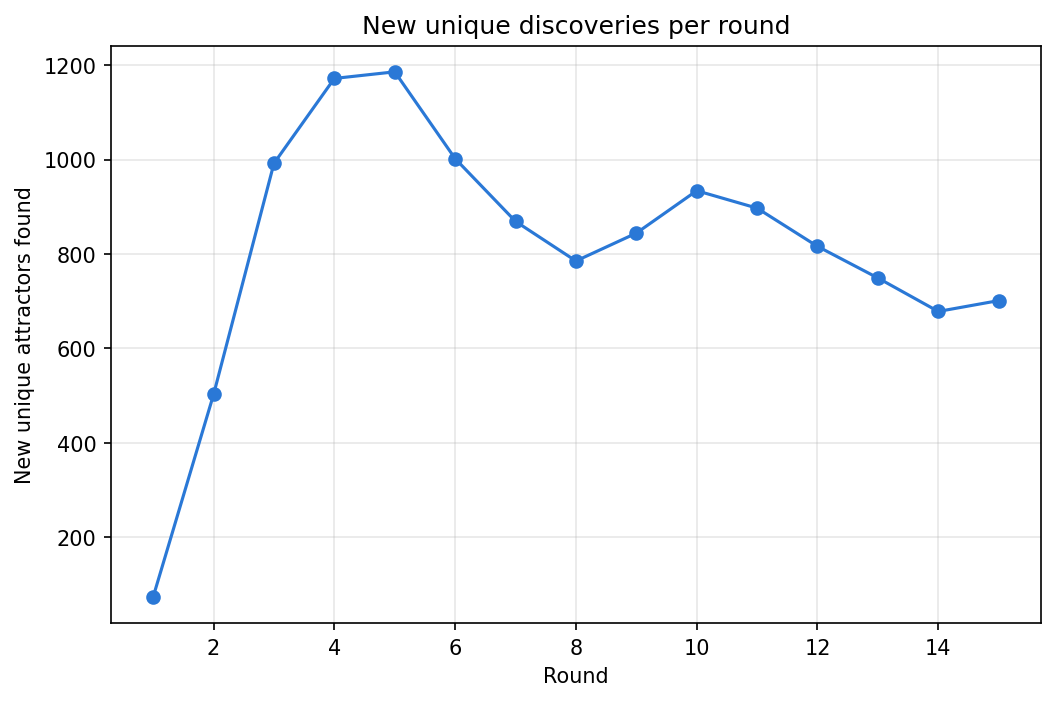
\includegraphics[width=0.75\linewidth]{figures/newHitsPerRound.png}
\caption{New, distinct chaotic discoveries per round (the \emph{Distinct}
column of Table~\ref{tab:rounds}). Yield rises sharply over rounds 1--4,
peaks at round 5, then decays through round 14 with a small uptick at round
15.}
\label{fig:taper}
\end{figure}

\begin{figure}[htbp]
\centering
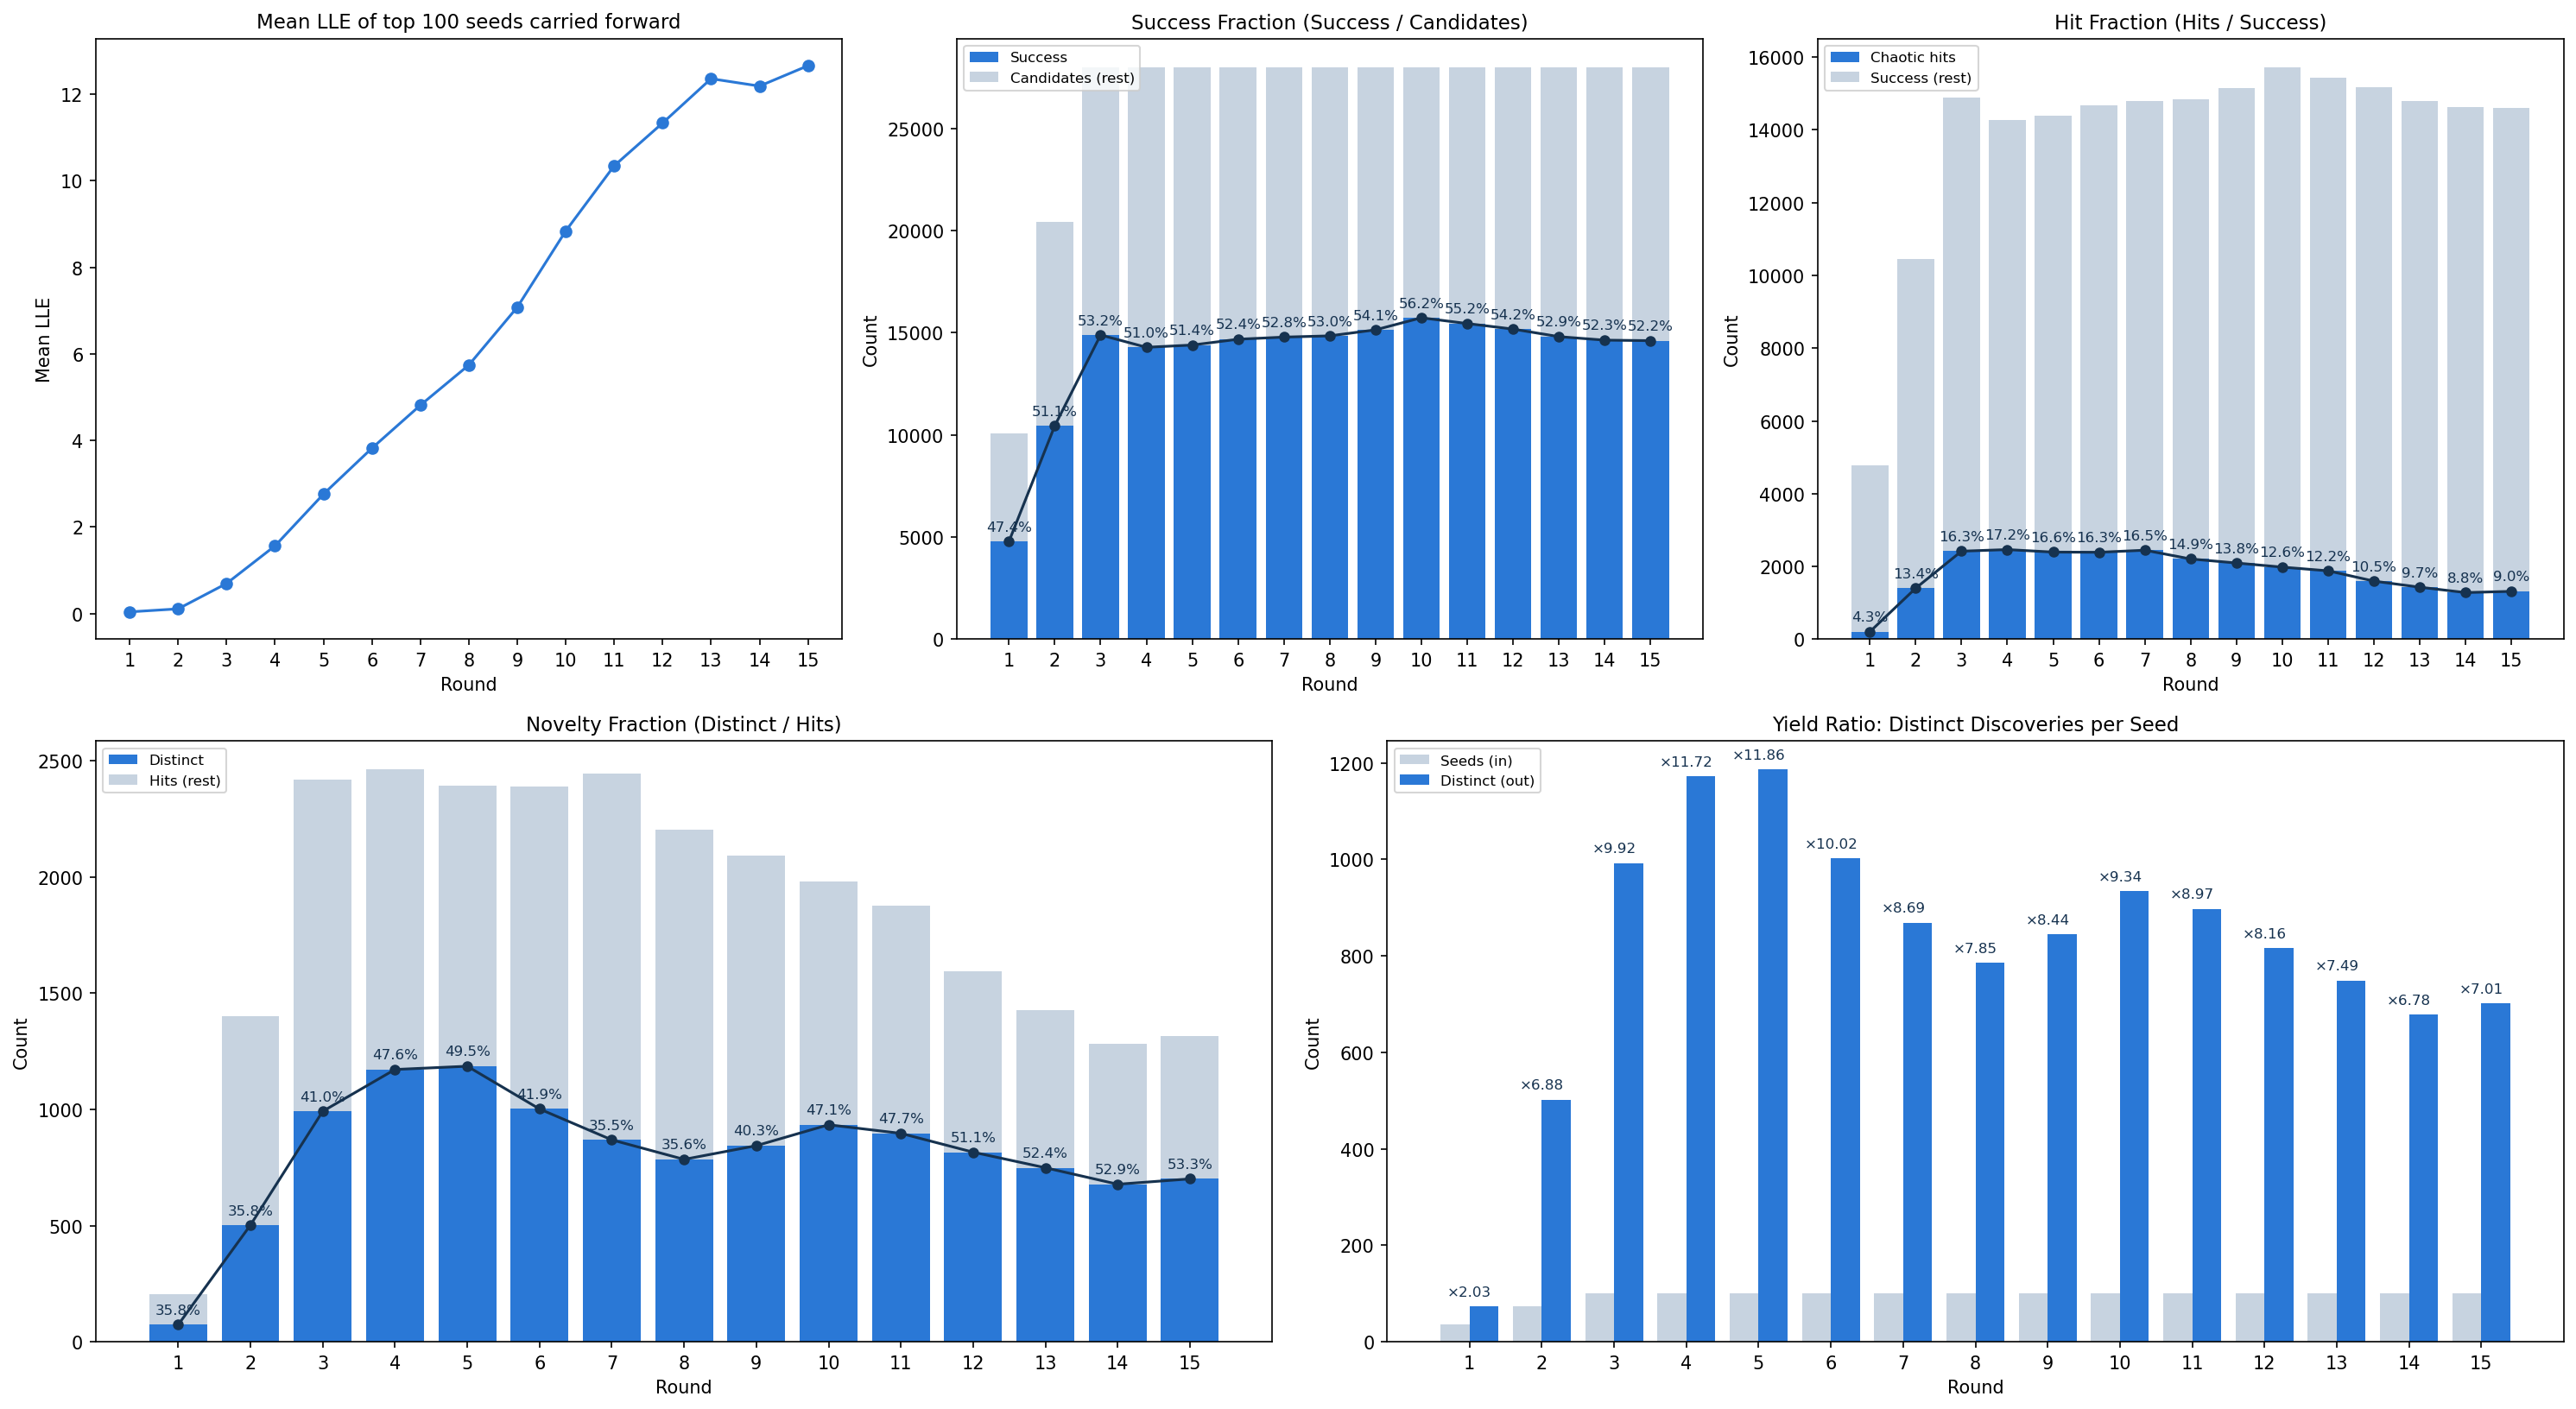
\includegraphics[width=\linewidth]{figures/roundDiagnostics.png}
\caption{Round-by-round diagnostics. Top row, left to right: mean fitness
(LLE) of the capped seed set carried into each round; the success fraction
(successfully integrated candidates over all candidates); the hit fraction
(chaotic hits over successfully integrated candidates). Bottom row: the
novelty fraction (distinct discoveries over chaotic hits); the yield ratio
(distinct discoveries produced per seed used that round).}
\label{fig:diagnostics}
\end{figure}

Across all 15 rounds, the framework evaluated 394{,}423 raw candidates
surviving the catalog-proximity filter, of which 208{,}634 (53\%) integrated
successfully, 27{,}496 (13\% of successes) were classified chaotic by the
chaos oracle, and 12{,}200 (44\% of chaotic hits) were confirmed distinct from
every other known or discovered system by the novelty oracle.

Several patterns in Table~\ref{tab:rounds} and Figures~\ref{fig:taper}--%
\ref{fig:diagnostics} are worth stating precisely before interpreting them in
\S\ref{sec:discussion}:

\begin{itemize}
  \item The catalog-proximity filter of \S3.5 removes at most 0.1\% of raw
  candidates in any of the 15 rounds (0--27 out of 28{,}000), despite the
  catalog itself growing past ten thousand points by round 15. Near-collisions
  with already-cataloged points remain rare at the radii used, even deep
  into the run, likely due to the sheer size of the search space.
  \item \emph{Hit Frac.} rises from 4.3\% (round 1) to a peak of 17.2\% (round
  4), then declines fairly steadily to 8.8\% (round 14), with a small uptick
  to 9.0\% at round 15.
  \item \emph{Novelty Frac.} rises from 35.8\% (rounds 1--2) to 53.3\%
  (round 15), with a mid-run dip
  to 35.5--41.9\% around rounds 6--8.
  \item The yield ratio (Distinct/Seeds) peaks at round 5 (11.86$\times$) and
  decays to a minimum of 6.78$\times$ at round 14. It never approaches
  $1\times$ anywhere in the reported window.
  \item Mean seed fitness (LLE) rises essentially monotonically across all 15
  rounds, from 0.04 to 12.66.
  \item Cross-oracle disagreement (the cascade's verdict differing from
  curvature's or D2's independent verdict, logged per round to
  \texttt{disagreements.csv}, \S\ref{sec:novelty-oracle}) is recorded for
  35--54\% of all chaotic hits in every round. This is a different, larger
  population than the 94.1\% figure in the Cascade calibration limitation,
  which is
  restricted to the subset of hits the cascade itself confirms distinct.
\end{itemize}

Beyond the fitness and yield dynamics above, the discovered systems'
coefficient structure itself shows a corresponding round-over-round trend.

\begin{table}[htbp]
\centering
\footnotesize
\caption{Round-over-round statistics of $|w_i|$, the absolute value of a
discovery's 81 normalized coefficients, averaged first within a discovery
and then over that round's distinct discoveries, computed from each
round's own authoritative result file. \emph{Std} is the standard deviation
of that per-discovery average across the round's discoveries; \emph{CV} =
$\frac{\mathit{Std}}{\mathit{Mean}}$.}
\label{tab:coefstructure}
\begin{tabular}{rrrr}
\toprule
Round & Mean $|w_i|$ & Std $|w_i|$ & CV \\
\midrule
1  & 0.039 & 0.012 & 0.294 \\
2  & 0.045 & 0.014 & 0.308 \\
3  & 0.060 & 0.020 & 0.344 \\
4  & 0.084 & 0.007 & 0.082 \\
5  & 0.085 & 0.005 & 0.059 \\
6  & 0.085 & 0.005 & 0.054 \\
7  & 0.086 & 0.004 & 0.049 \\
8  & 0.086 & 0.005 & 0.053 \\
9  & 0.083 & 0.005 & 0.063 \\
10 & 0.080 & 0.004 & 0.050 \\
11 & 0.079 & 0.003 & 0.041 \\
12 & 0.078 & 0.002 & 0.029 \\
13 & 0.078 & 0.002 & 0.029 \\
14 & 0.078 & 0.002 & 0.024 \\
15 & 0.078 & 0.002 & 0.026 \\
\bottomrule
\end{tabular}
\end{table}

Since every system has unit $\ell_2$ norm (\S\ref{sec:representationOfSearchSpace}), Mean
$|w_i|$ measures how evenly a discovery's coefficient mass is spread across
the 81 monomials versus concentrated in a few. The corresponding
\emph{signed} mean (not shown) stays within $\pm 0.03$ across all 15
rounds, an order of magnitude smaller, so Table~\ref{tab:coefstructure} is
not merely tracking a sign bias. Two patterns stand out. First, the mean
itself rises sharply over rounds 1--3 (0.039 to 0.060) before jumping to a
plateau around 0.084--0.086 by round 4, then declining gradually to 0.078
by round 15 -- the same round-4 transition visible in
Table~\ref{tab:rounds}'s fitness and yield statistics. Second, and more
strikingly, the coefficient of variation collapses from 0.29--0.34 in
rounds 1--3 to 0.02--0.08 from round 4 onward: the \emph{population} of
discoveries within a round, not just the typical discovery, becomes
substantially more homogeneous in this structural sense as soon as the
beam's top-100 capping takes hold, an independent, structural echo of the
same selection-driven narrowing already visible in Table~\ref{tab:rounds}'s
monotonically rising mean seed LLE.

Table~\ref{tab:rounds} and Figures~\ref{fig:taper}--\ref{fig:diagnostics}
characterize the run in aggregate. Figure~\ref{fig:discoveries} shows what a
handful of the individual discoveries driving those statistics actually
look like.

\begin{figure}[htbp]
\centering
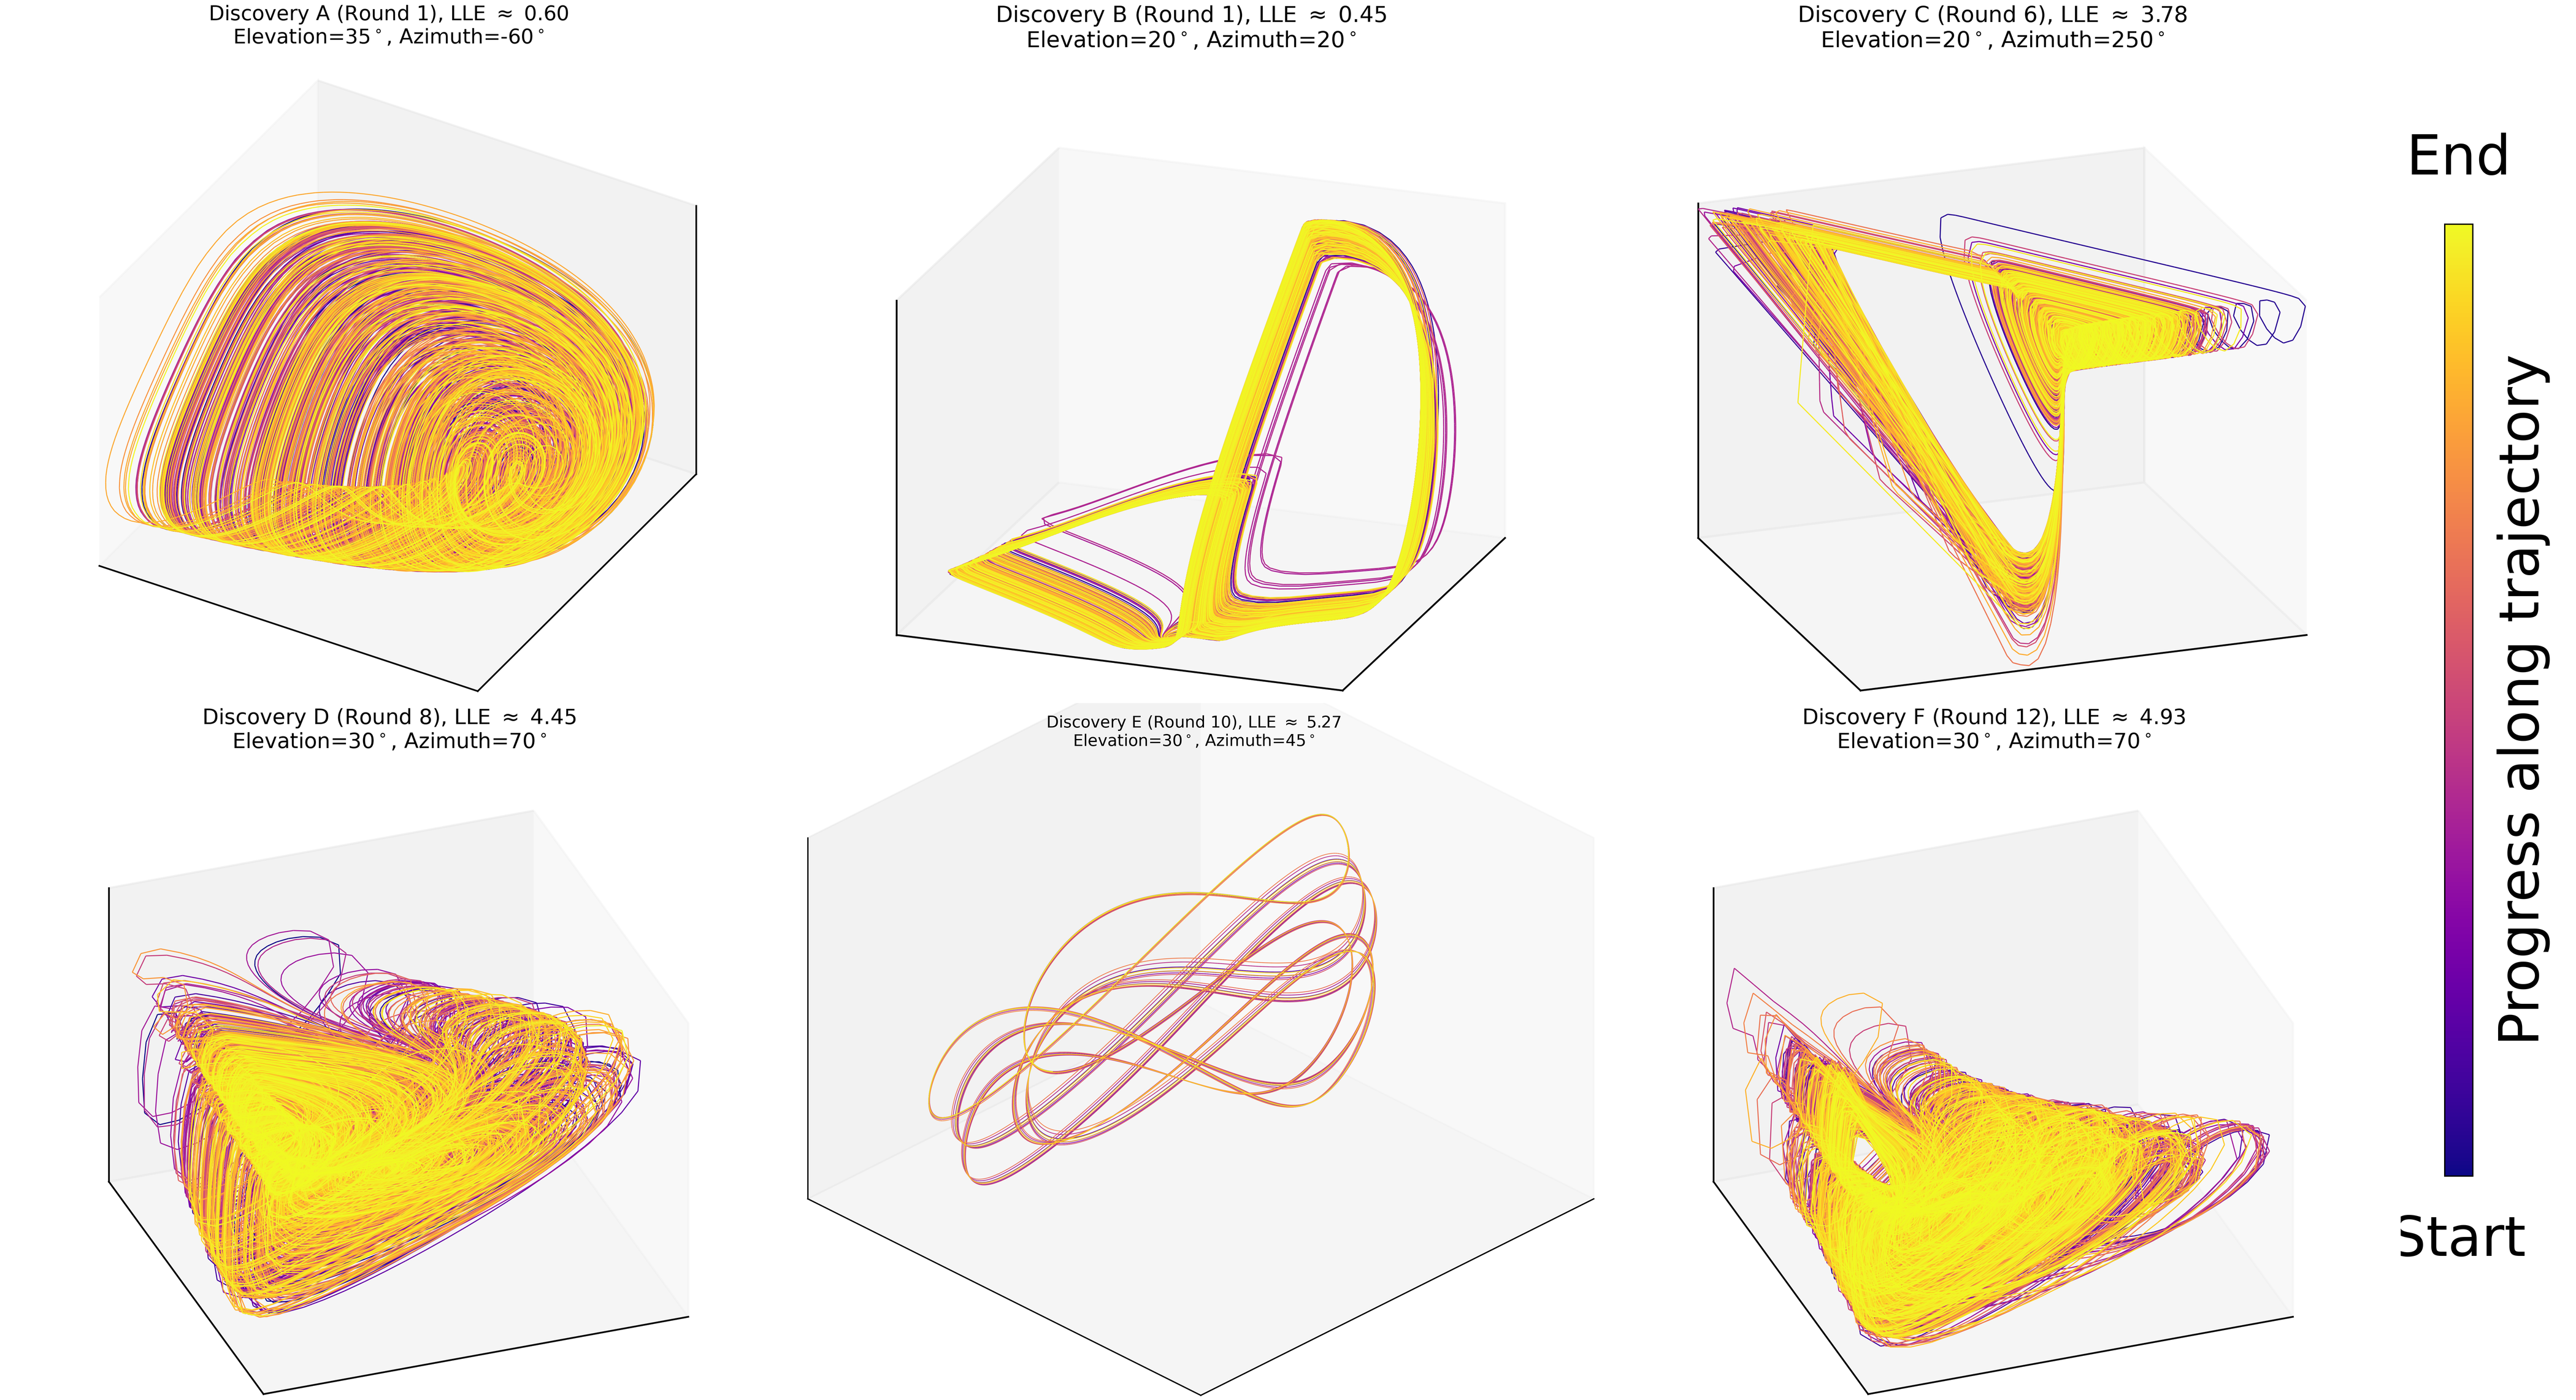
\includegraphics[width=\linewidth]{figures/discoveredAttractors.png}
\caption{Six discoveries from the reported run (Discoveries A--F; internal
labels and originating round: A~=~NewHit\_68, round~1; B~=~NewHit\_60,
round~1; C~=~NewHit\_3980, round~6; D~=~NewHit\_6143, round~8;
E~=~NewHit\_7753, round~10; F~=~NewHit\_9756, round~12), chosen for visual
variety rather than as a representative sample. Each was also necessarily
drawn from the subset of discoveries with a saved trajectory, which is
itself biased toward lower LLE, as stated in the ``Trajectory-save success
declines with LLE'' discussion. Each panel plots the
system's own real saved trajectory (not an idealization); color encodes
progress along that trajectory from start to end. An orthographic (not
perspective) projection is used throughout to preserve each trajectory's
true shape, and each panel's viewing angle was chosen individually to
exemplify that system's structure. Every system shown was independently
verified to remain bounded and chaotic under a from-saved-endpoint re-integration run
20 times longer than the originally saved window, rather than relied on
from the chaos oracle's classification alone (\S\ref{sec:chaos-oracle}). D
and F -- discovered independently thirteen rounds apart -- are shown from
the same viewing angle to allow direct comparison.}
\label{fig:discoveries}
\end{figure}

\section{Discussion}
\label{sec:discussion}

\paragraph{Early transient.} The sharp rise in \emph{Novelty Frac.} alongside
the sharp rise in \emph{Hit Frac.} over rounds 1--4 plausibly reflects a
transient effect of starting from a small, curated, scientifically
interesting (rather than densely representative) seed set of 36 named
attractors, before the beam-capping rule's selection pressure settles into a
steadier regime around round 5--6.

\paragraph{The Hit Fraction decline.} As the seed population becomes increasingly
selected for extreme fitness (mean LLE), nearby candidates become
\emph{less}, not more, likely to test chaotic under the chaos oracle. The
blowup/stability precheck failure rate stays roughly flat (44--53\%) across
the entire run, so this effect is concentrated specifically in the ``succeeds
numerically but is not chaotic'' outcome, not in outright integration
failure. We flag this as an open empirical pattern rather than a settled
mechanism: we have not independently established \emph{why} the immediate
geodesic neighborhood of a strongly chaotic system becomes less likely to be
itself chaotic as the seed pool's mean fitness rises, only that the
pipeline's own logs show this correlation holding consistently across ten or
more consecutive rounds.

\paragraph{The Novelty Fraction rise.} That \emph{Novelty Frac.} rises over the same
span is at minimum consistent with -- though does not on its own prove -- the
catalog-proximity filter (\S\ref{sec:Catalog-proximity-filtering}) increasingly doing more of the ``has this
territory been seen before'' work as the catalog grows, leaving the
shape-based novelty oracle (\S\ref{sec:novelty-oracle}) to adjudicate an
increasingly pre-filtered, spatially separated population of candidates.

\paragraph{Yield does not collapse within 15 rounds.} The yield ratio decays
from its round-5 peak but stays well above $1\times$ through round 15
(Table~\ref{tab:rounds}), meaning the search was still finding, on average,
roughly seven new distinct chaotic systems for every seed used as late as
round 14 and round 15. Nothing in the reported window indicates the locally reachable
novel territory around the current beam is close to exhausted. Whether yield
eventually approaches a floor is a question for longer runs, not one this
15-round window can answer.

\paragraph{Trajectory-save success declines with LLE.}
\label{sec:trajectory-save-bias}
The pipeline saves a
full integrated trajectory for each distinct discovery as a final, separate
step after classification and novelty-checking are complete, and this step
did not always succeed or run to completion. Whether it did is directly
checkable in the released output, by matching each catalog row's round and
label against the saved trajectory files for that round. Of the 12{,}200
distinct discoveries, 6{,}506 (53.3\%) have a saved trajectory and 5{,}694
(46.7\%) do not. The save rate itself falls from 98.6\% in round 1 to
roughly 20\% by round 15, and the two populations differ sharply in fitness
-- mean LLE 0.81 among discoveries with a saved trajectory versus 5.01
among those without.
Whatever makes trajectory-saving more likely to fail, it does not act
uniformly across the catalog: it selectively removes the most strongly
chaotic discoveries from the saved-trajectory subset. Any figure or
qualitative description built from saved trajectories, including
Figure~\ref{fig:discoveries}, is therefore drawn from a population biased
toward the catalog's less extreme half, not a representative cross-section
of it.

\section{Limitations}
\label{sec:limitations}

\paragraph{No incentive toward sparsity.}
\label{sec:sparsity-limitation}
Counting nonzero entries directly
in the seed dataset's own coefficient file and the released catalog's: the
55 known systems of \S\ref{sec:seeds} average only 6.8 of 81 nonzero
coefficients (Lorenz itself has 7, \S\ref{sec:representationOfSearchSpace}). By contrast, every
one of the 12{,}200 discovered systems is fully dense, with none having a
single coefficient closer than $10^{-6}$ to zero. Geodesic stepping has no mechanism
that favors sparse directions, and neither the chaos nor the novelty oracle
penalizes density, so a discovery's 81-term polynomial can carry many
small-magnitude terms that contribute little to the actual trajectory but
clutter the equation and add cost to every downstream computation that
touches it (integration, descriptor evaluation, novelty comparison): a mean
of 18 (median 15) of a discovery's 81 coefficients fall below $|w_i| =
0.02$ in magnitude without ever reaching zero. Future work could bias the
equiangular direction set itself toward sparser regions of the sphere, or
apply a post-hoc rounding step that zeros out coefficients below a
validated no-visible-effect threshold, trading a small amount of
geometric precision for substantially simpler equations, closer to the
sparsity of the named attractors this search was seeded from.

\paragraph{Limited integration time in classification.} The chaos oracle's
accept/reject decision is based on 3--5 draws, each integrated for a fixed
simulated time of $1000/\mathrm{scaleBy}$ (\S\ref{sec:chaos-oracle}),
enough to separate genuine chaos from the great majority of non-chaotic
candidates, but not all of them. Preparing Figure~\ref{fig:discoveries}
surfaced direct evidence of the gap: among the high-fitness candidates
considered for that figure, five were confirmed, under a
from-saved-endpoint re-integration 20 times longer than the classification
window, to actually be a fixed point or a finite-time blowup rather than a
genuine chaotic attractor: false positives the oracle's fixed-length window did
not catch. Three of those five had already been accepted into the catalog
and used as seeds for subsequent rounds before this was discovered
(NewHit\_5601, NewHit\_10961, and NewHit\_5314, propagating to 3, 1, and 9
child discoveries respectively, counted directly from the released
catalog's own \emph{ParentLabel} field). Because the oracle's integration window
is, by construction, blind to any instability that only manifests later,
some unknown number of the 12{,}200 cataloged systems are likely to be
further false positives of the same kind, not only the five identified
during figure preparation.

\paragraph{Fixed search geometry.} Direction count (40), the set of used
radii (seven fixed values), beam width (100), and the
backward/sideways distance threshold (one-half of a candidate's own
generating radius)
were each chosen once, informed by compute-budget considerations, and held
fixed for the entire reported run. The yield dynamics in
\S\ref{sec:results} are properties of the search \emph{as configured}, not
demonstrated to be universal properties of the underlying coefficient space
independent of that configuration.

\paragraph{Fitness-driven selection bias.} Because the chaos
oracle's fitness score is also the beam's ranking criterion, the seed
population at every round beyond the second is deliberately not
representative of ``typical'' chaotic systems. It is biased toward the most
strongly chaotic tail by construction (the monotonic mean-LLE rise in
Table~\ref{tab:rounds} is a direct, expected consequence of this rule, not an
independent discovery about the dynamics). The resulting 12{,}200-system
catalog oversamples strongly chaotic dynamics relative to what an unranked or
randomly-capped beam would have produced. This matters for any use of the
catalog's current composition to make a population-level statistical claim
about how common chaos is among triquadratic polynomial vector fields in
general.

\paragraph{Cascade calibration beyond the original catalog.}
\label{sec:cascade-calibration-limitation}
The released catalog records each discovery's distance to its nearest
reference under all three methods, and the numbers below come from those
recorded distances. Curvature and D2 disagree with the cascade's
``distinct'' call on 94.1\% of the 12{,}200 discoveries, almost always
together rather than independently (70.7\% of all discoveries). Part of
this is built into how the novelty oracles were validated in the first place:
known chaotic attractors are traditionally given names only when they can be 
told apart from other attractors, usually by the human eye.
As such, the self/cross-distance test (\S\ref{sec:novelty-oracle}), which
uses these known attractors, is effectively a test of visual distinctness.
The cascade, which relies on both visual information from multiple angles
to shortlist candidates and rigid alignment of the trajectories' own point
clouds to make the actual decision, measures this visual distinctness
directly. On the other hand, curvature and D2 measure correlated but
different statistical summaries, and score worse on that same test
(false-positive 22.2\% vs 11.1\%, false-negative 36.1\% vs 11.1\%). This is
also why the cascade, not curvature or D2, makes the actual accept/reject
decision. A separate,
more open question is scale: that calibration was measured by comparing the
original 36 known attractors to each other, but by round 15, 99.5\% of a
discovery's nearest match is another discovery from this run, not one of
those 36. Almost every real decision late in the run is checked against a
large, almost-entirely self-generated population the cascade's threshold was never tested
against, and whether it holds up as well there is left open.

\section{Applications}

\paragraph{Forecasting and modelling benchmarks.} The catalog extends
existing curated benchmark collections \citep{gilpin2021chaos,gilpin2023model}
by roughly two orders of magnitude in system count, with the important
caveat (above) that its current LLE distribution is not representative of
generic chaotic dynamics and should be accounted for, not ignored, in any
benchmark use.

\paragraph{Data-driven system identification.} System identification is the
reverse of simulation: instead of starting from known equations and
generating trajectory data, it starts from observed trajectory data and
tries to recover the governing equations that produced it. Sparse
system-identification methods such as SINDy \citep{brunton2016discovering}
search for a sparse combination of candidate monomial terms that
reproduces observed data, and evaluating such a method requires comparing
its recovered coefficients against the true, known equations that
generated the data. Discovered systems come with exact, known ground-truth
polynomial coefficients, making them suitable test cases for this purpose
at a scale well beyond the handful of classical named systems typically
used for it. One caveat is relevant here: the ``No incentive toward
sparsity'' limitation notes that every
discovered system is fully dense, unlike the sparse ground truth SINDy is
designed to recover. Many of a discovery's coefficients are small in
magnitude, however, without ever reaching zero. This makes the catalog a natural test of how such methods
behave when the true system is only approximately, not exactly, sparse.
This is a realistic regime for noisy real-world data, one the classical
named systems cannot test since they are sparse by construction. Because
so many of these small coefficients are negligible without being exactly
zero, a large fraction of discoveries could likely be converted to
genuinely sparse ground truth via the post-hoc rounding step that same
limitation describes, trading a small amount of precision for
ground truth closer to what SINDy is built to recover. The reverse
direction already holds in this pipeline: SINDy-adjacent tooling
\citep{stevenshaas2024genexperiments} converts \emph{known} systems into the
representation this search explores (\S\ref{sec:seeds}). So the discovered
catalog closing the loop back into system-identification benchmarking would
extend an already-used dependency to a new purpose, not introduce one.

\paragraph{Reuse of the framework with other oracles.} Because the search
framework is oracle-agnostic (\S\ref{sec:modularity}), the same procedure could
target other objects of interest within the same or a different polynomial
family by substituting the oracles. For example, changing the chaos oracle we used into a bifurcation-boundary
detector or a target-Lyapunov-spectrum-shape detector, and/or substituting
the novelty oracle for a topological or symbolic-dynamics-based distinctness
criterion -- without any change to \S\ref{sec:representationOfSearchSpace}--\ref{sec:Catalog-proximity-filtering} or \S\ref{sec:capping}.

\paragraph{The search as its own probe.} Independent of its output catalog,
running the framework is itself an empirical probe of the local structure of
whatever region of coefficient space it is pointed at: the persistently low
catalog-collision rate and the non-collapsing yield ratio reported in
\S\ref{sec:results} are observations about that structure, obtainable from
running the framework with any chaos/novelty oracle pair, not only the
specific pair used to produce this paper's catalog.

\section{Conclusion}

Geodesic Beam Search adapts beam search, a general state-space search
strategy \citep{bisiani1987beam}, to continuous polynomial vector field
space: it expands a frontier of candidate systems via equiangular geodesic
steps, filters out re-exploration of known territory, and caps the next
round's frontier to the fittest recent discoveries, while remaining agnostic
to the specific rules used to decide what counts as chaotic and what counts
as new. Over 15 rounds, starting from 36 known chaotic attractors, this
produced 12{,}200 systems confirmed geometrically distinct from everything
else known or discovered, out of roughly 394{,}000 candidates evaluated. The
search's own yield dynamics are, we argue, as much a result of this work as
the catalog itself: an early transient, a sustained but decaying yield
ratio that never approaches exhaustion within the reported window, and a
monotonic fitness-selection drift that is a direct consequence of the
beam-capping rule rather than an independent finding.

Future work includes: longer runs to determine whether yield eventually
approaches a floor or a different steady regime; adaptive radius schedules in
place of the fixed set used here; concretely substituting alternative chaos
and novelty oracles to test the modularity claim of \S\ref{sec:modularity}
directly, rather than only arguing for it structurally; formally
separating the fitness criterion from the chaos oracle into its own
independent fitness oracle, since nothing in the framework requires the
two to be computed together; and a population-level
statistical characterization of the 12{,}200-system catalog (Lyapunov spectra, bifurcation
structure) as a follow-up paper in its own right. Finding an
efficient, well-calibrated novelty oracle was itself one of the harder parts
of this work (\S\ref{sec:novelty-oracle}), a difficulty also discussed in
the Cascade calibration limitation, and a
better one would likely improve the method's results substantially. But
what counts as ``better'' depends on what notion of similarity the oracle is
meant to prioritize (shape difference, visual difference, or some other
criterion entirely). Which notion best fits a given research goal is itself
an open question this paper does not settle.

\section*{Code and Data Availability}

The implementation of Geodesic Beam Search described in this paper, together
with the full discovery catalog from the 15-round run reported in
\S\ref{sec:results}, will be released as open-source software at
\url{https://github.com/Isaac-L-D/geodesic-beam-search} upon publication.
Per-round discovery trajectories and explored tangent directions, too large
to host in the code repository itself, are archived on Zenodo at
\url{https://doi.org/10.5281/zenodo.23856993}.

\section*{AI Assistance Disclosure}

Claude (Anthropic), via Claude Code, was used to assist with both the
software implementation described in this paper and the writing of the
paper itself, under the direction and review of the human authors.

\bibliographystyle{plainnat}
\bibliography{references}

\end{document}
